\chapter{Research}


\section{History}

In 1736, \citet{euler} solved the Seven Bridges of Ka\"{o}nigsberg problem by drawing a graph.
\citet{ismail2009some}
\todo{a strange paper to choose. perhaps multiple citations?}
pinpoint his use of this method as the birth of graph theory.

Graph theory has many applications to modelling the real world \ldots

\subsection{Tutte-embeddings}

In 1963, \citet{tutte} popularised [says who] the problem of graph drawing when he presented 

["who showed that polyhedral graphs may be drawn in the plane with all faces convex by fixing the vertices of the outer face of a planar embedding of the graph into convex position, placing a spring-like attractive force on each edge, and letting the system settle into an equilibrium"]

This contained two important ideas: embeddings(, , and the application of an attractive spring-like attractive force \ldots 

\subsection{Knuth}

In the same year, \citet{Knuth63} described a system for drawing flowcharts that describe algorithms. \citet{battista} \todo{find out page number!} says this is [the first example of an algorithm for visualising information] although \citeauthor{Knuth63} cites earlier work done on a similar system by \citet{haibt1959}.

\citet{Knuth63} does not describe his flowcharts as graphs, but 

The annual symposium is 


\ldots

\citet{huang2007effects} divide graphs into two groups: abstract graphs and domain graphs.
GSN arguments fall into the latter category \ldots  therefore \ldots
\todo{I don't think this is widely agreed upon}




\section{What makes a good graph layout?}

The GSN was intended to be a clearer way of presenting arguments than free text.
The process of breaking down arguments into their constituent parts achieves some of this clarity,
but the notation's graphical nature also appears to be important.
This raises the question of whether the particular layout of graphs can affect their comprehensibility.

Some attempts have been made to enumerate the vital characteristics of a good graph layout, often in order to understand the trade-offs between different algorithms running times and the quality of the layouts produced.


\subsection{Quality metrics}

\citet{Himsolt95comparingand} compared a total of 11 different graph layout algorithms, ranging from force directed to more specialised ones only suitable for particular categories of graph (such as planar and directed acyclic).
As well as running time, and six quantitative layout-related criteria -- ranked in order of significance after observing the layouts produced -- there is included a ``personal rating'' (on a scale of 1--5), based on the judgements of colleagues upon viewing the layouts produced.
However, details of the experimental method used, and detailed statistical results, are not provided.
\todo{Some o -- force directed algorithms produce good layouts for general graphs, but have the worst running time; DAG is also good with a better running time -- }

\citet{DiBattista1997303} compared four algorithms, providing more detailed results.
Improving on \citeauthor{Himsolt95comparingand}'s use of about 100 graphs, and earlier work \todo{can't find the paper (``S. Jones, P. Eades, A. Moran, N. Ward, G. Delott and R. Tamassia, A note on planar graph drawing algorithms, Technical Report 216, Department of Computer Science, University of Queensland (1991).'') they cite} that used purely randomly generated graphs, they took 112 graphs from real-word applications and generated 11,582 variations in total. They used implementations of the algorithms to lay out these graphs, and evaluated the resulting layouts according to nine quality metrics:

\begin{description}
    \item[Area]
``area of the smallest rectangle with horizontal and vertical sides covering the drawing''
    \item[Cross]
total number of edge crossings
    \item[TotalBends]
total number of edge bends
    \item[TotalEdgeLen]
total length of all edges
    \item[MaxEdgeBends]
``maximum number of bends on any edge''
    \item[MaxEdgeLen]
``maximum length of any edge''
    \item[UnifBends]
``standard deviation of the number of bends on the edges''
    \item[UnifLen]
``standard deviation of the edge length''
    \item[ScreenRatio]
``deviation from the optimal aspect ratio, computed as the difference between the width/height ratio of the best of the two possible orientations (portrait and landscape) of the drawing and the standard 4/3 ratio of a computer screen. ''
\end{description}

They boldly assert: ``It is widely accepted \ldots that small values of the above measures are related to the perceived aesthetic appeal and visual effectiveness of the drawing.''
However, being widely accepted does not always preclude being wrong.

The \textbf{ScreenRatio} metric is the least robust.
In general, the ideal aspect ratio will depend on various factors, such as where the graph is displayed.
Since the paper was published, data such as those published by Unity Technologies\footnote{\url{http://stats.unity3d.com/}} have shown that 4:3 is no longer the most common computer screen aspect ratio.
Standard paper sizes have a different aspect ratio still.
If aesthetic beauty is important, then perhaps the golden ratio \todo{reference} should be used instead.
However, being only one metric of nine, ScreenRatio has not been given undue significance, and it highlights a relevant point: linear layouts \todo{there should be a page in Di Battista's book}, for example, are likely to be difficult to fit into typical spaces.


\subsection{Evaluating quality metrics/human testing}

As graph theory, and in turn graph layout, has a broad range of applications, it follows that the reasons for giving significance to different aesthetic qualities can vary depending on the application.

For example, there can be many practical motivations for minimising edge crossings.
When P\`{a}l Tur\`{a}n worked in a brick factory during World War II,
he considered the minimum number of crossings in a graph representing
brick kilns, storage sites and the paths between them \todo{cite. and this is probably redundant fluff}.
Where a graph represents an electrical circuit, edge crossings affect how the circuit can be printed on a circuit board.
Clearly, none of these are relevant to laying out a graph to convey information.\todo{not quite right; graphs always \emph{convey information} but\ldots variations in the nature of the information being conveyed?} / these applications are very different to the layout of GSN arguments.

\citet{5674033} observe that ``Many graph layout algorithms that have been devised over
several decades have typically been designed in accordance with the intuitions of the algorithm designers.'' [So] attempts have been made to validate these intuitions.

First, particular aesthetics have been evaluated. \citet{Purchase1997basis} evaluated three -- symmetry, number of edge crossings, and number of edge bends -- by Then \citet{Purchase1997which} d


\citet{PURCHASE1998647} later evaluated whole algorithms

\ldots


Most recently, \citet{5674033} invited users to draw graphs :
compared ``formal'' (like the Artoo tool) and ``sketch'' interface modes.
interesting conclusion



\subsection{Gestalt principles}

The Gestalt principles of visual perception,
based on the wider Gestalt theory of the mind developed by German psychologists of the Berlin School in the late 19th and early 20th centuries,
are often applied to visual design and grap.

The principle 

The relationship between the Gestalt principles and \ldots can seem hazy and tenuous





\subsection{The human gold-standard \todo{this is part of the method, arguably}}

Building [sort of?] on the ideas in \cite{5674033}, one understanding of the ideal layout of a GSN argument can be reached by observing the layouts of arguments found ``in the wild''\todo{although it is not always clear whether these have been layed out ``manually'' or automatically}.
Plenty of material can be found in literature, for example in \cite{Habli:2006:PPC:1183088.1183090} and  \cite{insilico} \ldots

Layouts typically follow the guidelines described in the GSN specification \citep[section~2.2, pp.~26--27]{gsnstandard}, \todo{``should I consistently call it a ''community standard [document]'' or something else?}
to ``enable the reader to perceive the logical flow of the argument being presented, and to enhance its readability.''
The specification suggests that arguments should flow down the page, starting with an abstract parent goal at the top, progressing downwards as this is refined into more concrete child strategies, goals and solutions -- this allows the hierarchy of the graph to be understood without looking at the directions of the connecting arrows.
Context, assumption and justification elements are placed to the sides, a positioning which reflects their semantic role.

Although the specification document does not fully justify its recommendations, they seem reasonable, but there there are instances of authors contravening them.

Figure~\ref{fig:aldencentral} shows \citet{royal} placing child strategies around a central claim, contrary to the top-down approach recommended; this is repeated in two other arguments in \cite[pp.~8--9]{royal} \todo{\url{http://www-course.cs.york.ac.uk/pcsw/LaTeX/lecture.pdf} says ``don't use this form as a noun'' but \url{http://www.ieee.org/documents/style_manual.pdf} (chapter V) seems to say it's OK}.
A rough visual observation highlights that it takes slightly longer to identify the top-level claim node, but the layout is more area-efficient, and the enclosing rectangle \todo{``minimum bounding box''?} [has a more useful aspect ratio].
The refinements of the strategies do mostly follow the standard guidance, continuing in a top-down (or bottom-up) order, and with context, assumptions and justifications placed at the sides, but the children of strategy 1.1.1.4 do not.

\begin{figure}
    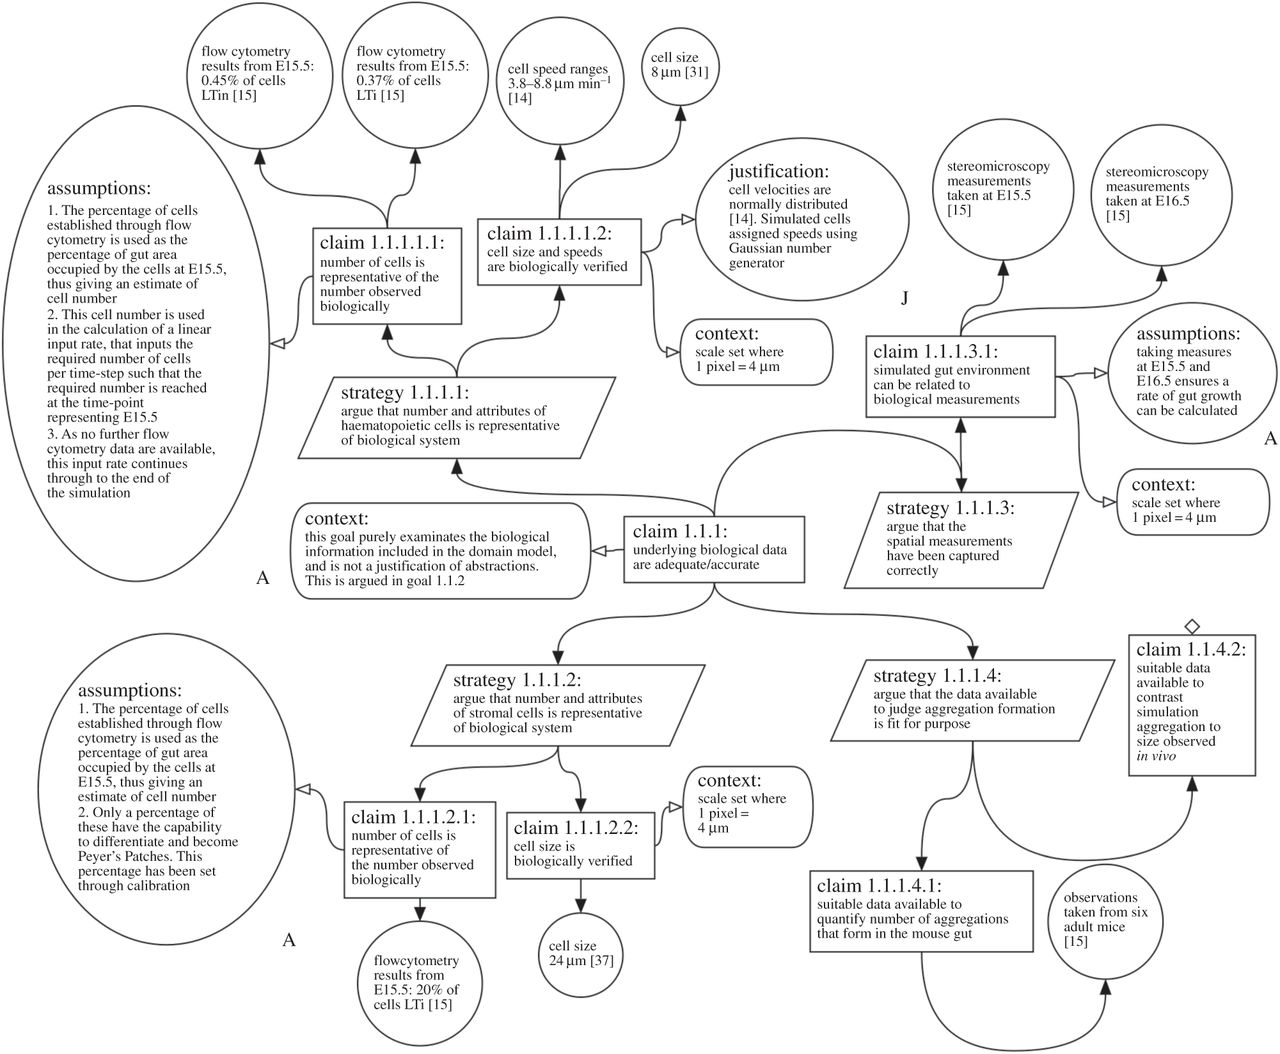
\includegraphics[width=\textwidth]{graphics/aldencentral.jpg}
    \caption{An argument from }
    \label{fig:aldencentral}
\end{figure}

In \cite{gsnstandard}, layout guidance is not demonstrated using specific diagrams, but there are many examples elsewhere in the document. These follow the guidelines, but are often imperfect in other ways:

\begin{itemize*}
\item As noted in section~\ref{sec:cramped}, the layout shown in figure~\ref{fig:crampedex1} is very dense.
\item Another example, shown in figure~\ref{fig:unalignedsiblings}, ignores \todo{I think ``violates'' would be wrong} Gestalt \ldots
\end{itemize*}

This supports a conclusion that, although examples found in literature are not always are perfectly laid out, the imperfections are at least easy to identify.

\begin{figure}
    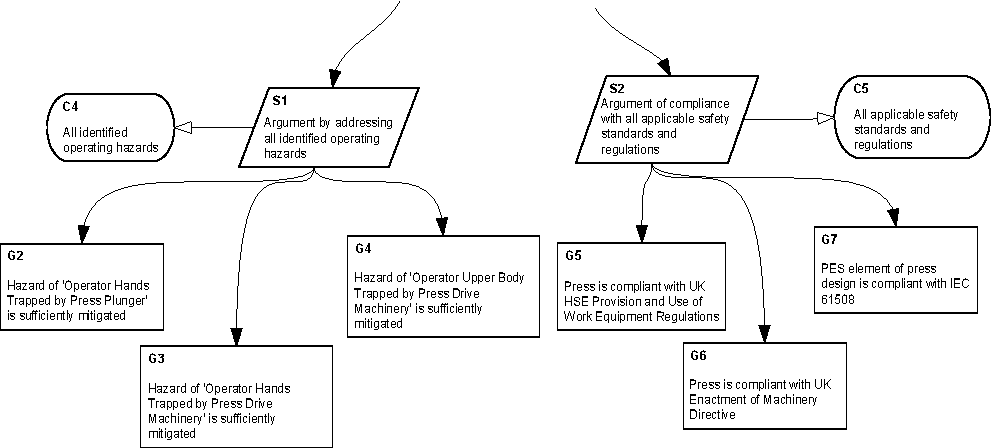
\includegraphics[width=\textwidth]{graphics/unaligned_siblings.pdf}
    \caption{A fragment of a GSN argument,
            from the GSN specification \citep[figure~42, section~2.3.6.5, pp.~34]{gsnstandard}}
    \label{fig:unalignedsiblings}
\end{figure}

\begin{figure}
    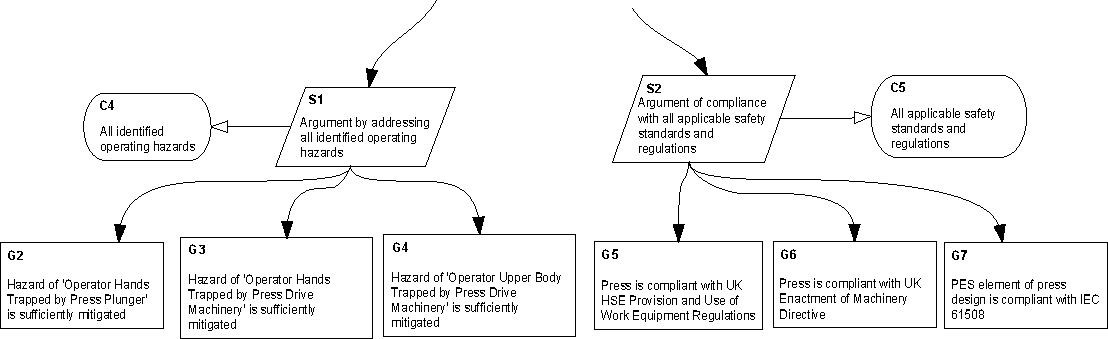
\includegraphics[width=\textwidth]{graphics/aligned_siblings.pdf}
    \caption{A modified version of figure~\ref{fig:unalignedsiblings},
            showing more clearly that the six goal elements are at the same level in the hierarchy}
    \label{fig:alignedsiblings}
\end{figure}



% \subsection{Edge crossings}


% [But] more relevantly [which studies?] have found that edge crossings is the most important factor for comprehension

% [who?] found that using the Gestalt principle of `closure' \ldots the viewer's mind instinctively joins up the lines




\section{Approaches to graph layout}

\subsection{Force directed algorithms}

Force directed graph layout algorithms are the descendants of \todo{as someone has observed?} \citet{tutte} \ldots a successor to \citet{tutte} spring embedding.

Force directed layout is simple to understand, being based on physical laws we encounter in the world 


[gansner 199*]

\subsection{grid}




\subsection{Layered graph drawing}

Layered or hierarchical graph drawing  \ldots sometimes generalised as Sugiyama's method, after \ldots who pioneered this technique \ldots 




\section{[GSN-/Artoo-specific considerations?]}

[move to Requirements?]

The  \ldots



\subsection{Dangling edges}

suggests incomplete graph

\subsection{Directed cycles}

It can be useful to remove directed cycles from the internal representation of a graph
(before drawing them back in their correct, original directions)
-- for example, in order to assign a consistent rank to each node.
This is achieved by reversing certain edges.
\citet{gansner1993} show that a simple depth-first-search \ldots  Minimising the number of edges is more difficult, \citeauthor{gansner1993} \ldots

\subsection{Undirected cycles}

Undirected cycles can be eliminated by ignoring certain edges altogether, to produce a tree.  [citation needed]








\section{Implementation}



The Artoo tool is written mainly in JavaScript, numerous different 

Various [things] have been developed in response to perceived shortcomings in JavaScript \ldots

Programs written in the CoffeeScript\footnote{\url{http://coffeescript.org/}} language, designed to be more succinct and with some extra features, can be transcompiled to JavaScript \ldots this is interesting but \ldots

Brython \footnote{\url{http://www.brython.info/}} is a Python 3 interpreter written in JavaScript that can run in a web browser. \todo{performance overhead etc\ldots}

Haste\footnote{\url{http://haste-lang.org/}}, UHC-JS\footnote{\url{http://uu-computerscience.github.io/uhc-js/}} and GHCJS\footnote{} are compilers from Haskell to JavaScript; SMLtoJS\footnote{\url{http://www.smlserver.org/smltojs/}} is a Standard ML--to-JavaScript compiler. These are perhaps most interesting [?], since \citet{kennedyfuntrees} observed that a tree layout algorithm implemented in Standard ML ``reflects the structure of the abstract solution much better than an imperative language implementation''.



ASM\footnote{} is a strict subset of 

[However]


\section{Software development methodologies}

In \citeyear{67poorslop}, \citet*{67poorslop} explained ``Why Programming is a Good Medium for Expressing Poorly Understood and Sloppily Formulated Ideas''
(More recently, [sussman] gave a talk with the same title \ldots \todo{\url{http://vimeo.com/12060509}}.)

This idea will be 

\section{}

Reuse of existing software libraries is widely [?] understood to be [a very sensible idea]. There are , which \ldots for comparison with 

\begin{description}
  \item[Springy] is 
  \item[Arbor] is an implementation of the Barnes-Hut algorithm described in  
  \item[The JavaScript InfoVis Toolkit] contains algorithms ported from \ldots
  \item[vis.js]
\end{description}

The Graphviz library contains several algorithms, including \ldots [as described in \ldots]. Although it is written in C, Emscripten \footnote{\url{http://emscripten.org}} can compile LLVM bitcode (readily compiled from C code) [as described earlier?] to the ASM subset of JavaScript -

These implementations also provide lessons on the structure of \ldots



agile
